\documentclass{article}
\usepackage[utf8]{inputenc}

% http://sourceforge.net/projects/pgfplots/
\usepackage{pgfplots}

\title{Automatic Word Clustering Generation}
\author{
  Mello, Ney\\
  \texttt{neymello@gwu.edu}
  \and
  Sá, Lucas\\
  \texttt{lucastsa@gwmail.gwu.edu}
  \and
  Silveira, José\\
  \texttt{silveiraneto@gwu.edu}
}
  \date{May 2013}

\usepackage{natbib}
\usepackage{graphicx}

\begin{document}

\maketitle

\section{Introduction}
There is a theory which states that if ever anyone discovers exactly what
 the Universe is for and why it is here, 
it will instantly disappear and be replaced by something even more bizarre 
and inexplicable. \citep{kowalski2011information}
There is another theory which states that this has already happened

\begin{figure}[h!]
\centering
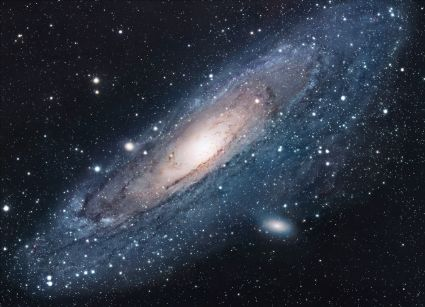
\includegraphics[scale=1.7]{universe.jpg}
\caption{The Universe}
\label{threadsVsSync}
\end{figure}

\section{A graph}
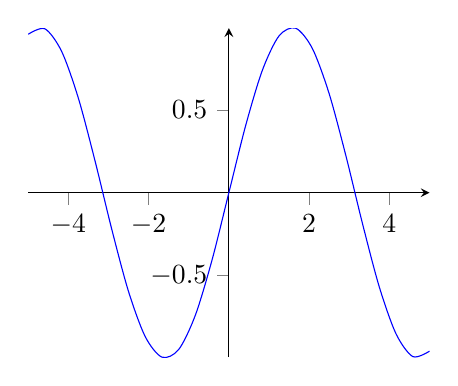
\begin{tikzpicture}
    \begin{axis}[width=190pt,axis x line=middle, axis y line=center, tick align=outside]
    	\addplot+[mark=none,smooth] (\x,{sin(\x r)});
	\end{axis}
\end{tikzpicture}

\section{Conclusion}
``I always thought something was fundamentally wrong with the universe'' \citep{adams1995hitchhiker}

\bibliographystyle{plain}
\bibliography{references}
\end{document}
